\section{Метод Эйлера}\label{sec:sol-euler}
Наивное интегрирование методом Эйлера:
\begin{equation}
    \mathbf S_{n+1} = \mathbf S_{n} + h\Delta{\mathbf S_n},
\end{equation}
где $h$ -- скорость в методе Эйлера, а
\begin{equation}
    \Delta{\mathbf S_n} = -|\gamma|\left[\mathbf S_n \times 
    \mathbf H^{eff}\right].
\end{equation}

Убедимся на графиках в том что энергия при интегрировании методом Эйлера не
сохраняется и в том что ошибка накапливается линейно, поскольку используемый
численный метод, как сказано выше имеет 1 порядок, построив график зависимости
ошибки от времени при различном шаге. График зависимости ошибки энергии от
времени для метода Эйлера изображен на рис.~\ref{fig:eulerEnergy}.

О модели мы знаем не только то что она должна сохранять энергию, но и то что
вектора спинов находятся на единичной сфере, поэтому сумма длин всех векторов
должна сохраняться, для метода Эйлера график зависимости ошибки длины векторов
спинов от времени изображен на рис.~\ref{fig:eulerLength}.
\begin{figure}[H]
    \centering
    \begin{subfigure}[b]{0.49\textwidth}
        \centering
        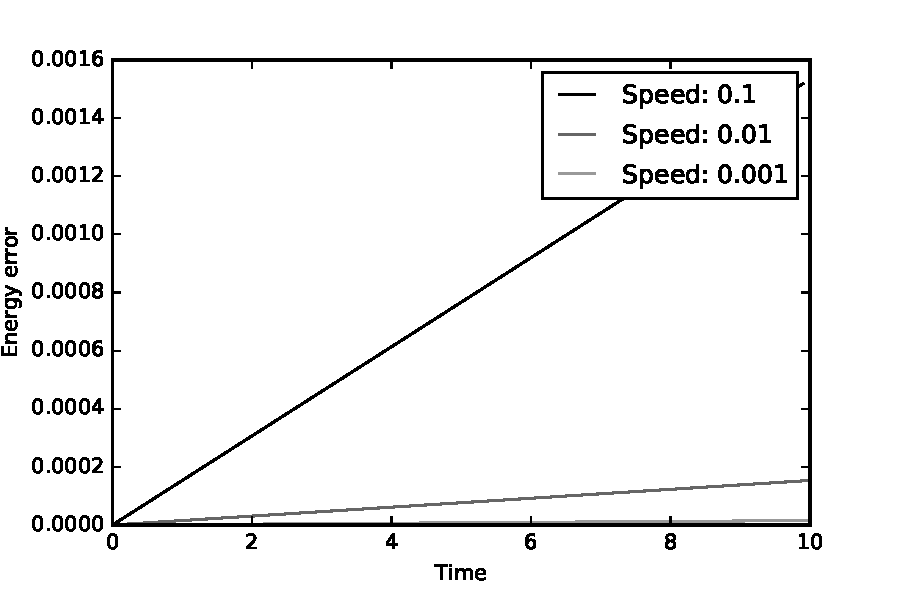
\includegraphics[width=\textwidth]{eulerEnergy.pdf}
        \caption{}
        \label{fig:eulerEnergy}
    \end{subfigure}
    \begin{subfigure}[b]{0.49\textwidth}
        \centering
        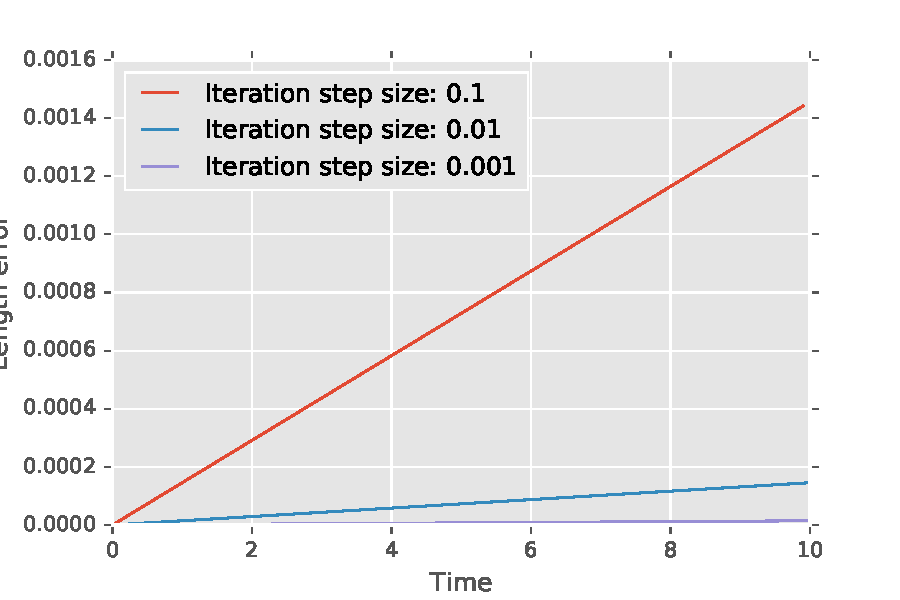
\includegraphics[width=\textwidth]{eulerLength.pdf}
        \caption{}
        \label{fig:eulerLength}
    \end{subfigure}
    \caption{(а) График зависимости ошибки энергии для метода Эйлера;
        (б) График зависимости ошибки суммы длин векторов спинов для
        метода Эйлера.}
\label{fig:euler-errors}
\end{figure}

%Для сохранения длины спинов можно на каждой итерации нормировать все вектора из
%$\mathbf S$.

%, тогда графики будут выглядеть как  и
 %для энергии системы и проекции векторов на
%направление магнитного поля соответственно.
